%UCD-1: Creazione artefatto

\begin{figure}
\centering
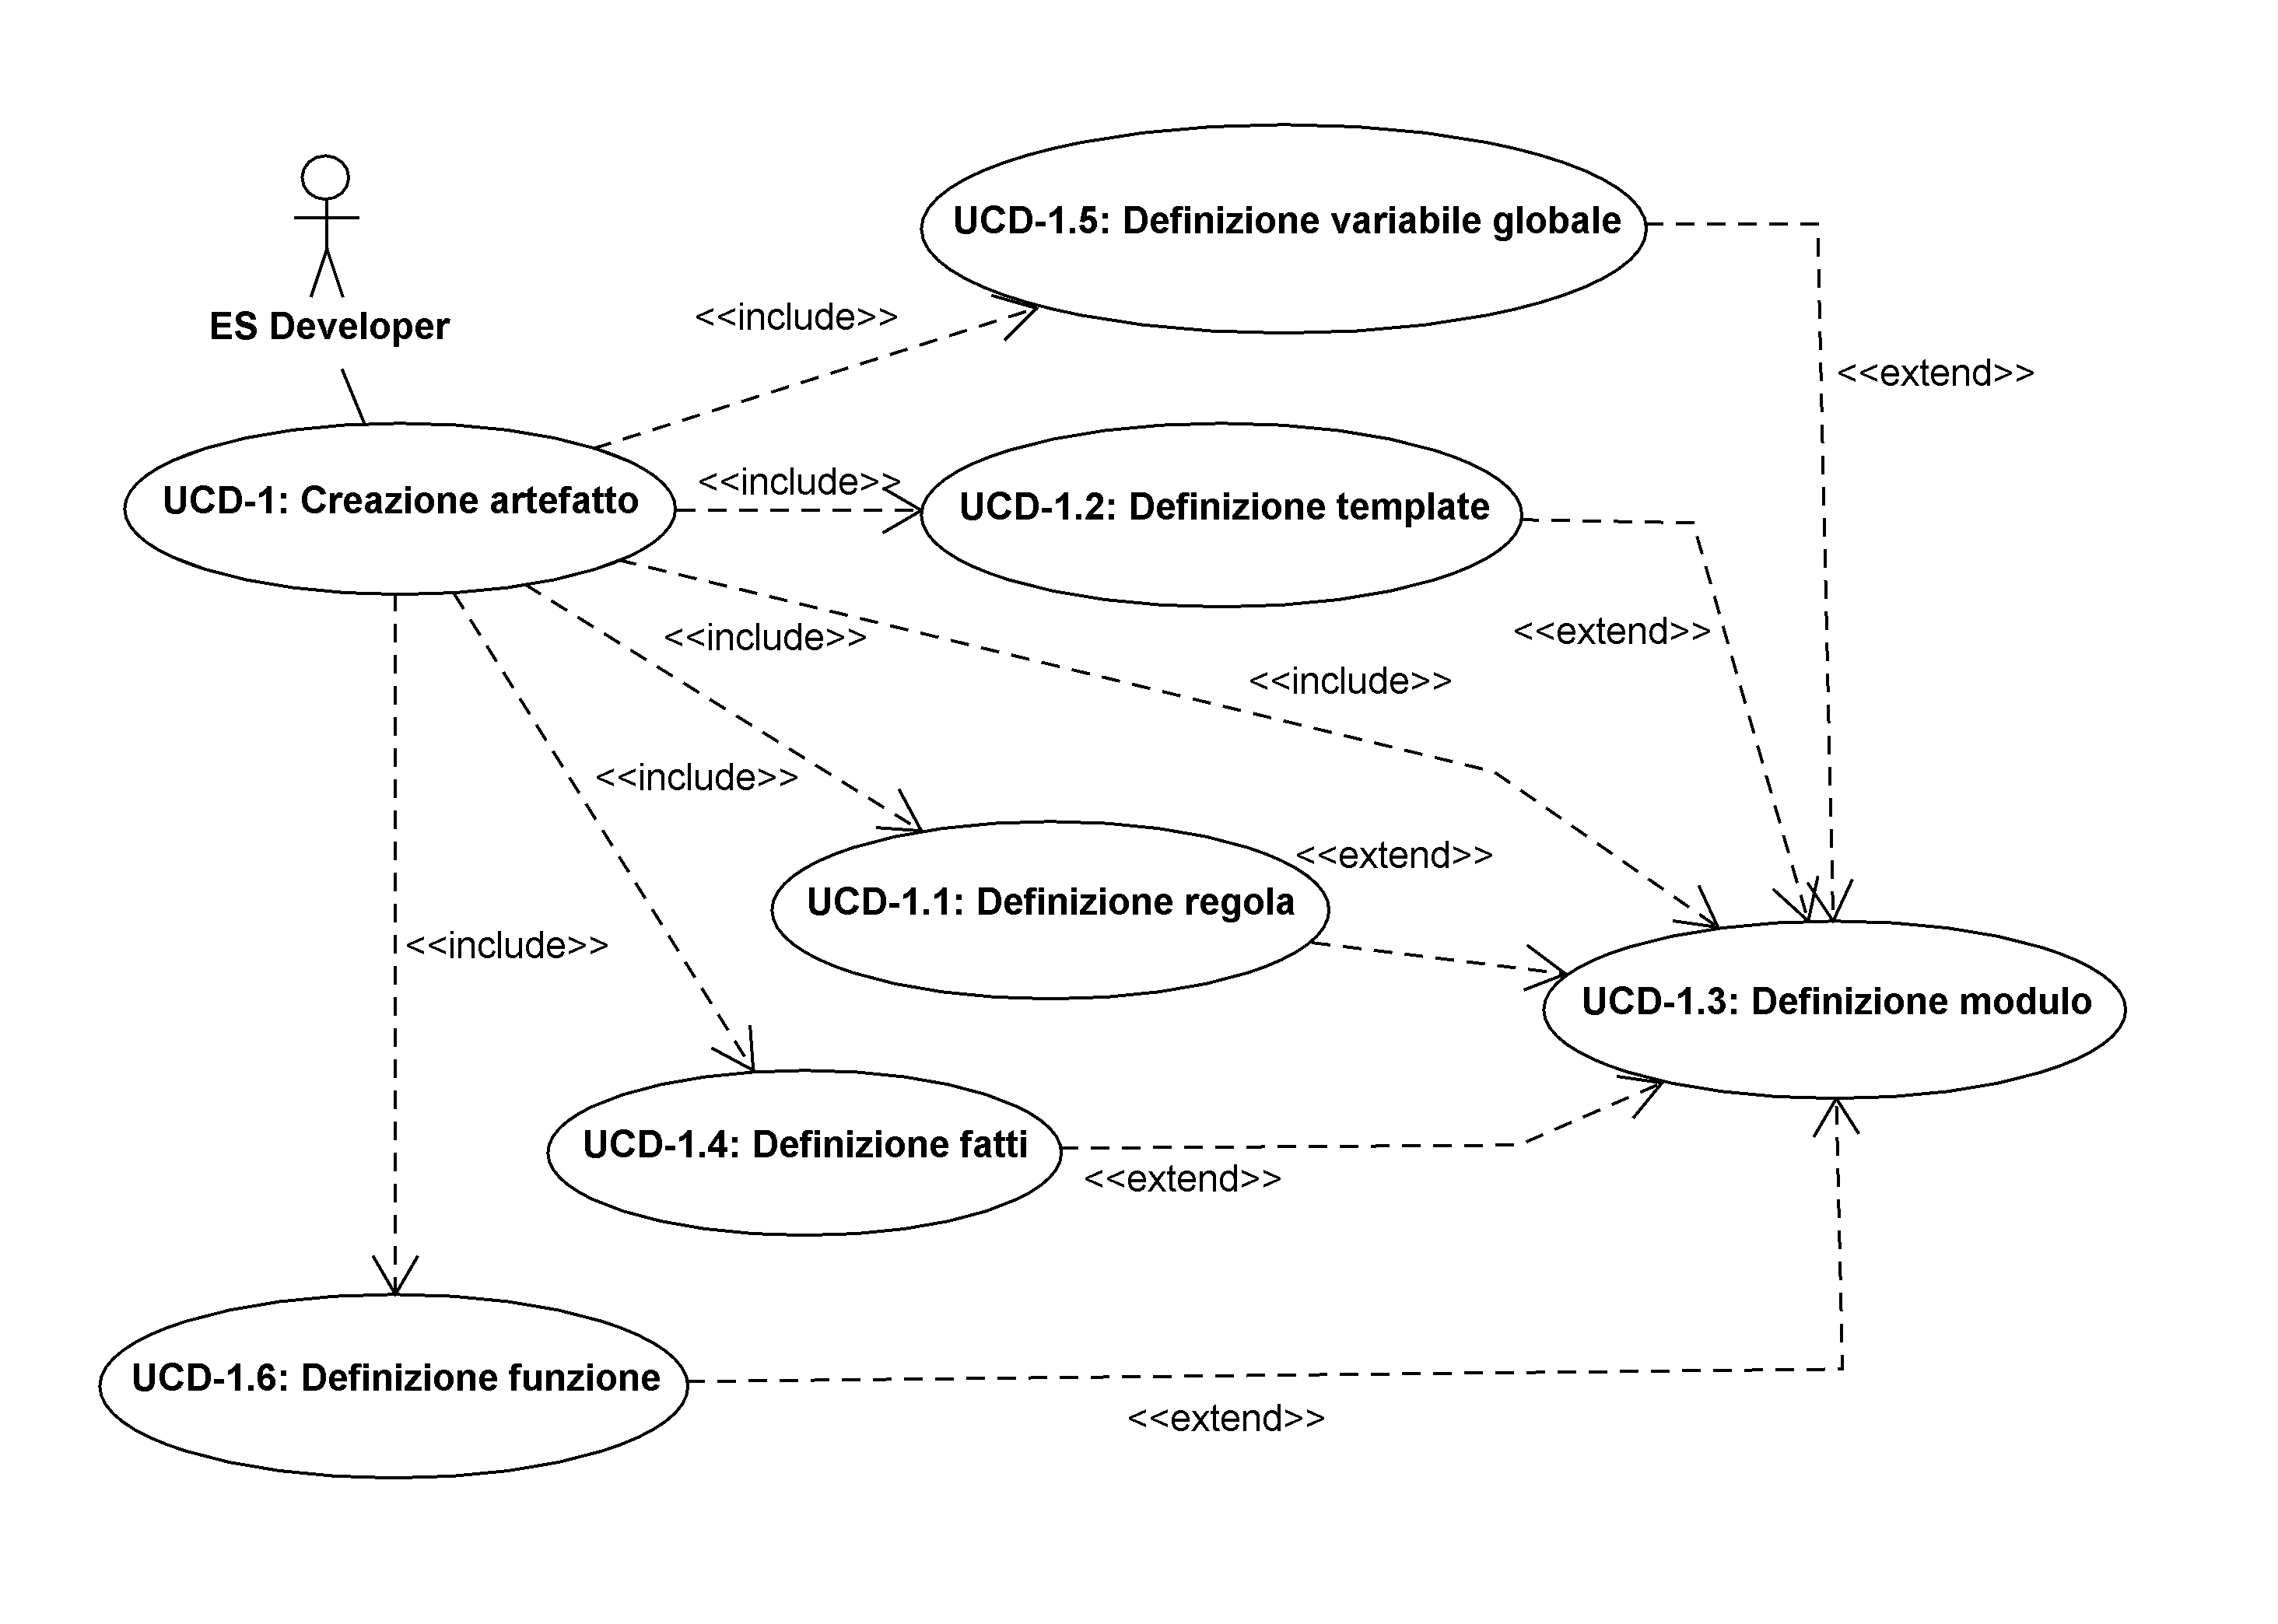
\includegraphics[width=1.1\textwidth]{Immagini/Capitolo2/UseCases/UCD-1.png}
\caption{Diagramma dei casi d'uso UCD-1}\label{fig:uc-ucd-1}
\end{figure}


\begin{itemize}
	\item \textbf{Attori:} ES Developer
	\item \textbf{Scopo e descrizione:} un ES Developer deve essere in grado di definire i costrutti necessari alla realizzazione di un artefatto.
	\item \textbf{Pre-condizioni:} il software fornisce almeno un linguaggio di specifica
	\item \textbf{Post-condizioni:} un artefatto è stato serializzato tramite il linguaggio di specifica
	\item \textbf{Flusso principale degli eventi:}
		\begin{enumerate}
			\item l'ES Developer definisce una serie di costrutti (si vedano i casi d'uso \emph{UCD-1.1}, \emph{UCD-1.2}, \emph{UCD-1.3}, \emph{UCD-1.4}, \emph{UCD-1.5}, \emph{UCD-1.6}).
			\begin{itemize}
				\item l'ES Developer può formalizzarlo in formato nativo
				\item l'ES Developer può formalizzarlo in formatto CLIPS
			\end{itemize}
			\item l'ES Consumer verifica la correttezza dell'artefatto (si veda il caso d'uso \emph{UCD-1.2}).
		\end{enumerate}
\end{itemize}


\paragraph{UCD-1.1: Definizione regola}

\begin{itemize}
	\item \textbf{Attori:} ES Developer
	\item \textbf{Scopo e descrizione:} un ES Developer deve essere in grado di definire una regola tramite un linguaggio di specifica fornito dal sistema.
	\item \textbf{Pre-condizioni:} il software fornisce almeno un linguaggio di specifica
	\item \textbf{Post-condizioni:} la definizione di una regola è stata aggiunta ad un artefatto
	\item \textbf{Flusso principale degli eventi:}
		\begin{enumerate}
			\item l'ES Developer definisce una regola
			\begin{itemize}
				\item l'ES Developer può formalizzarli in formato nativo
				\item l'ES Developer può formalizzarli in formatto CLIPS
			\end{itemize}
		\end{enumerate}
	\item \textbf{Flusso alternativo:}
		\begin{enumerate}
			\item se l'ES Developer ha definito precedentemente un modulo, l'ES Developer può definire una regola come componente del modulo.
		\end{enumerate}
\end{itemize}


\paragraph{UCD-1.2: Definizione template}

\begin{figure}[h]
\centering
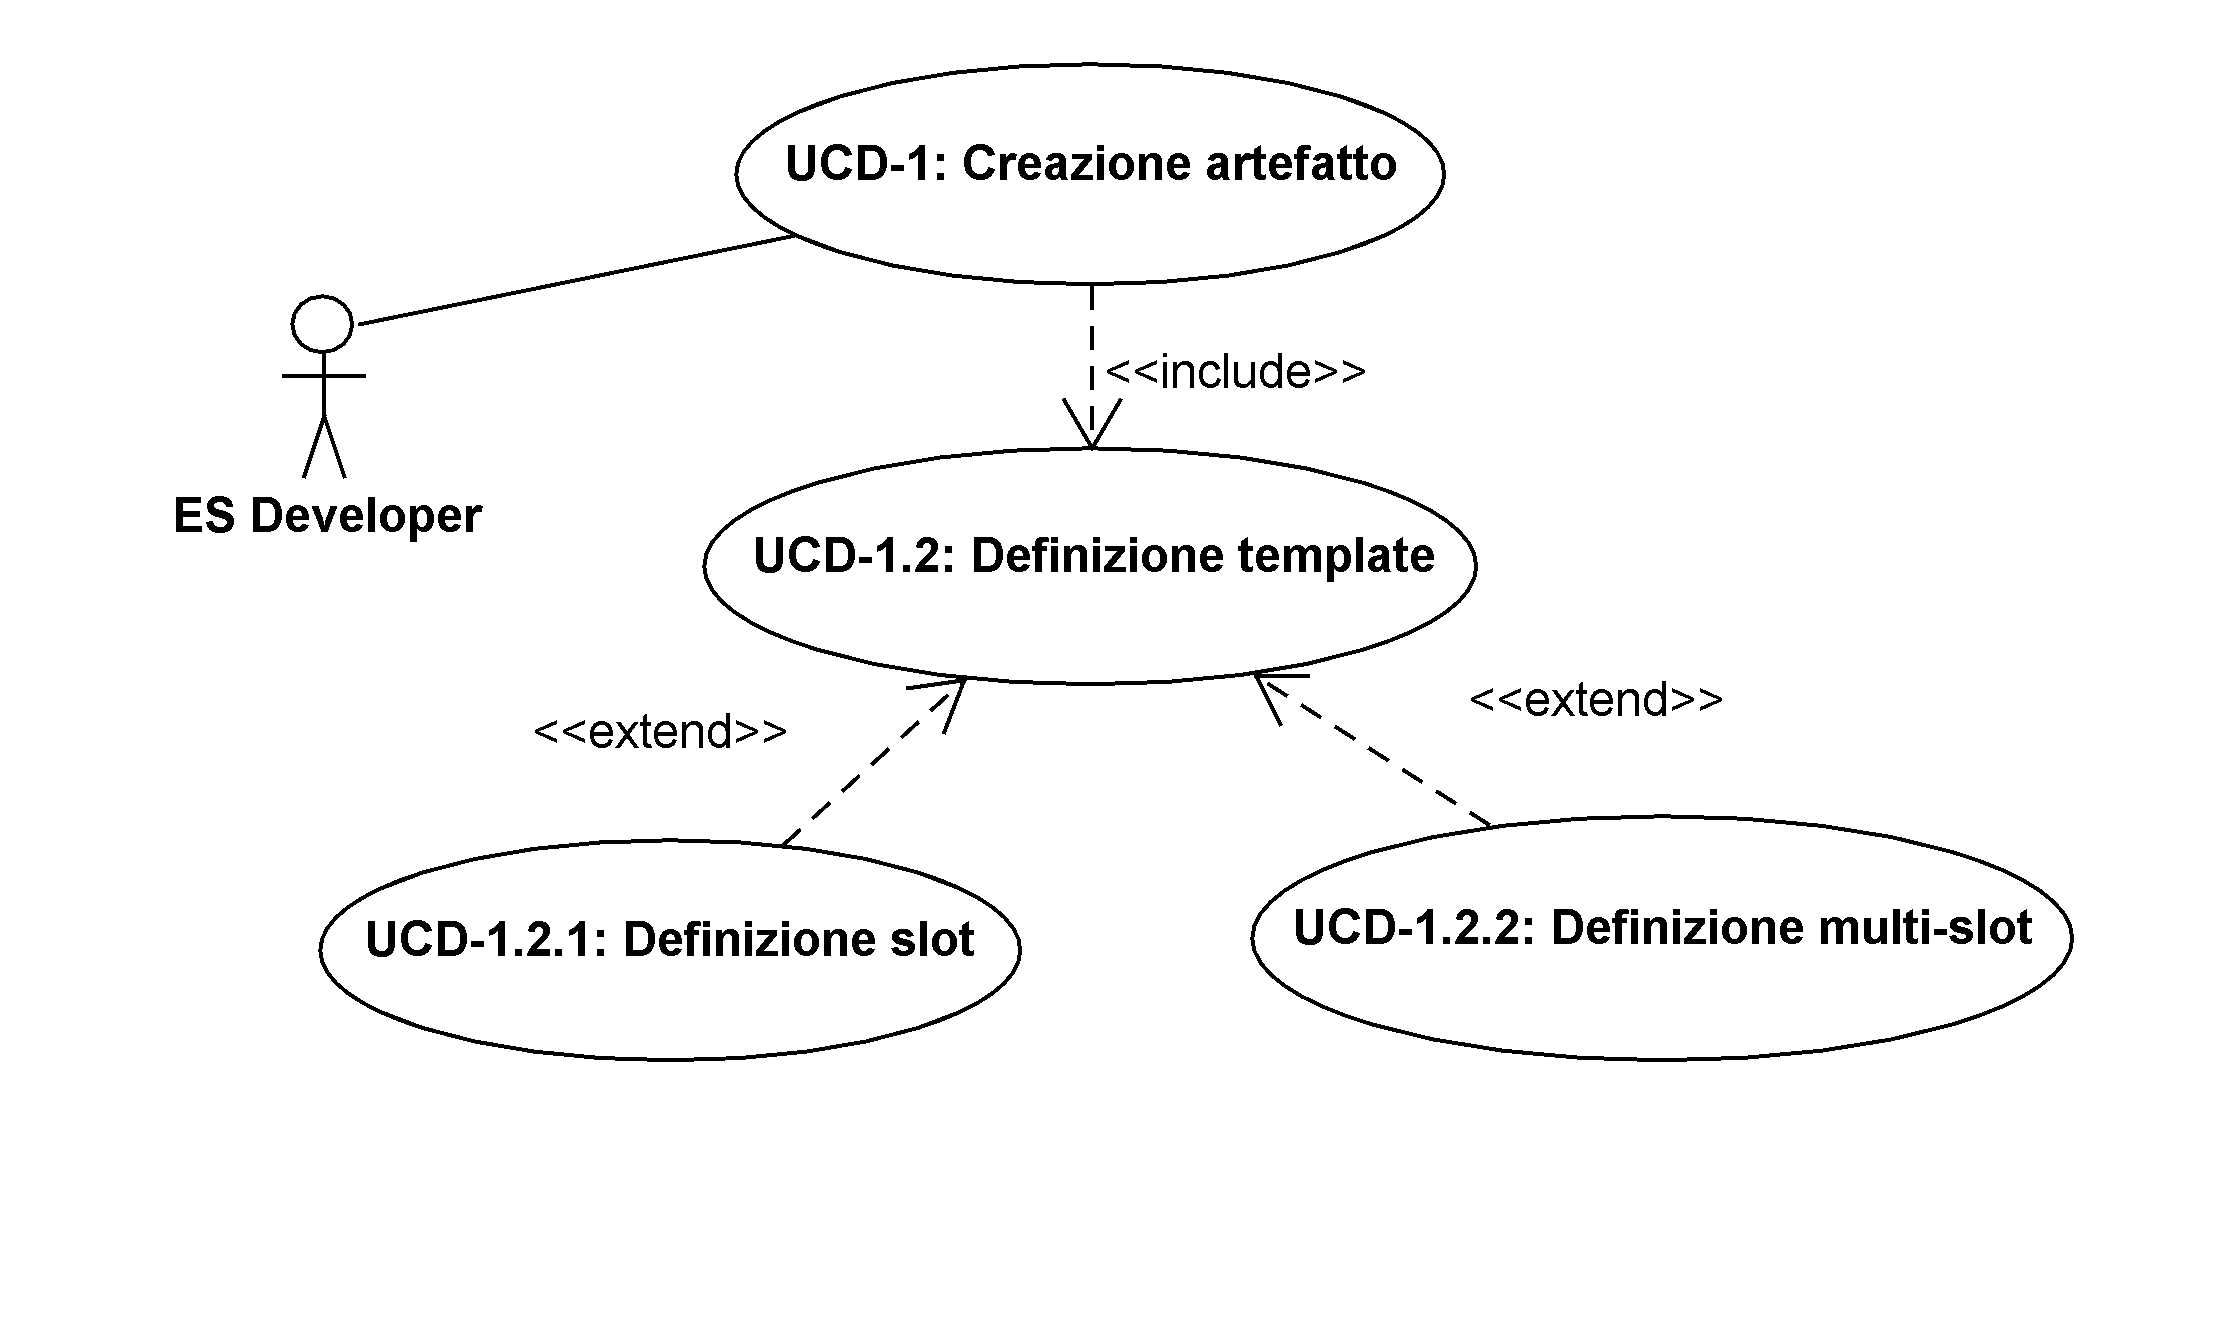
\includegraphics[width=1\textwidth]{Immagini/Capitolo2/UseCases/UCD-1_2.png}
\caption{Diagramma dei casi d'uso UCD-1.2}\label{fig:uc-ucd-1.2}
\end{figure}

\begin{itemize}
	\item \textbf{Attori:} ES Developer
	\item \textbf{Scopo e descrizione:} l'ES Developer deve essere in grado di definire un template di fatti tramite un linguaggio di specifica fornito dal sistema.
	\item \textbf{Pre-condizioni:} il software fornisce almeno un linguaggio di specifica.
	\item \textbf{Post-condizioni:} la definizione di un template di fatti è stato aggiunto ad un artefatto
	\item \textbf{Flusso principale degli eventi:}
		\begin{enumerate}
			\item l'ES Developer definisce un template di fatti
			\item l'ES Developer definisce il formato del template di fatti (si vedano i casi d'uso \emph{UCD-1.2.1}, \emph{UCD-1.2.2})
		\end{enumerate}
	\item \textbf{Flusso alternativo:} 
		\begin{enumerate}
			\item se l'ES Developer ha definito precedentemente un modulo, l'ES Developer può definire un template di fatti come componente di un modulo
		\end{enumerate}
\end{itemize}

\subparagraph{UCD-1.2.1: Definizione slot}

\begin{itemize}
	\item \textbf{Attori:} ES Developer
	\item \textbf{Scopo e descrizione:} l'ES Developer deve essere in grado di definire il formato di uno slot appartenente ad un template di fatti
	\item \textbf{Pre-condizioni:} il software fornisce un linguaggio di specifica, l'ES developer ha definito un template di fatti
	\item \textbf{Post-condizioni:} il formato dello slot è stato aggiunto alla definizione di template di fatti
	\item \textbf{Flusso principale degli eventi:}
		\begin{enumerate}
			\item l'ES Developer definisce un template
			\item l'ES Developer definisce un nuovo slot fornendo il nome (stringa alfanumerica) da attribuire allo stesso
			\begin{enumerate}
				\item l'ES Developer può definire una restrizione di tipo al contenuto dello slot
				\item l'ES Developer può definire un valore di \emph{default} per lo slot
			\end{enumerate}
		\end{enumerate}
	\item \textbf{Flusso alternativo:} 
		\begin{enumerate}
			\setcounter{enumi}{1}
			\item se l'ES Developer ha fornito un nome già usato da un altro slot o multi-slot presente, il sistema rifiuta la definizione notificando un errore.
		\end{enumerate}
\end{itemize}

\subparagraph{UCD-1.2.2: Definizione multi-slot}

\begin{itemize}
	\item \textbf{Attori:} ES Developer
	\item \textbf{Scopo e descrizione:} l'ES Developer deve essere in grado di definire il formato di un multi-slot appartenente ad un template di fatti
	\item \textbf{Pre-condizioni:} il software fornisce un linguaggio di specifica, l'ES Developer ha definito un template di fatti
	\item \textbf{Post-condizioni:} il formato del multi-slot è stato aggiunto alla definizione di template di fatti
	\item \textbf{Flusso principale degli eventi:}
		\begin{enumerate}
			\item l'ES Developer definisce un template
			\item l'ES Developer definisce un nuovo multi-slot fornendo il nome (stringa alfanumerica) da attribuire allo stesso
			\begin{enumerate}
				\item l'ES Developer può definire delle restrizioni di tipo al contenuto dello slot
				\item l'ES Developer può definire dei valori di \emph{default} per il multi-slot
			\end{enumerate}
		\end{enumerate}
	\item \textbf{Flusso alternativo:} 
		\begin{enumerate}
			\setcounter{enumi}{1}
			\item se l'ES Developer ha fornito un nome già usato da un altro slot o multi-slot presente, il sistema rifiuta la definizione notificando un errore.
		\end{enumerate}
\end{itemize}


\paragraph{UCD-1.3: Definizione modulo}

\begin{figure}[h]
\centering
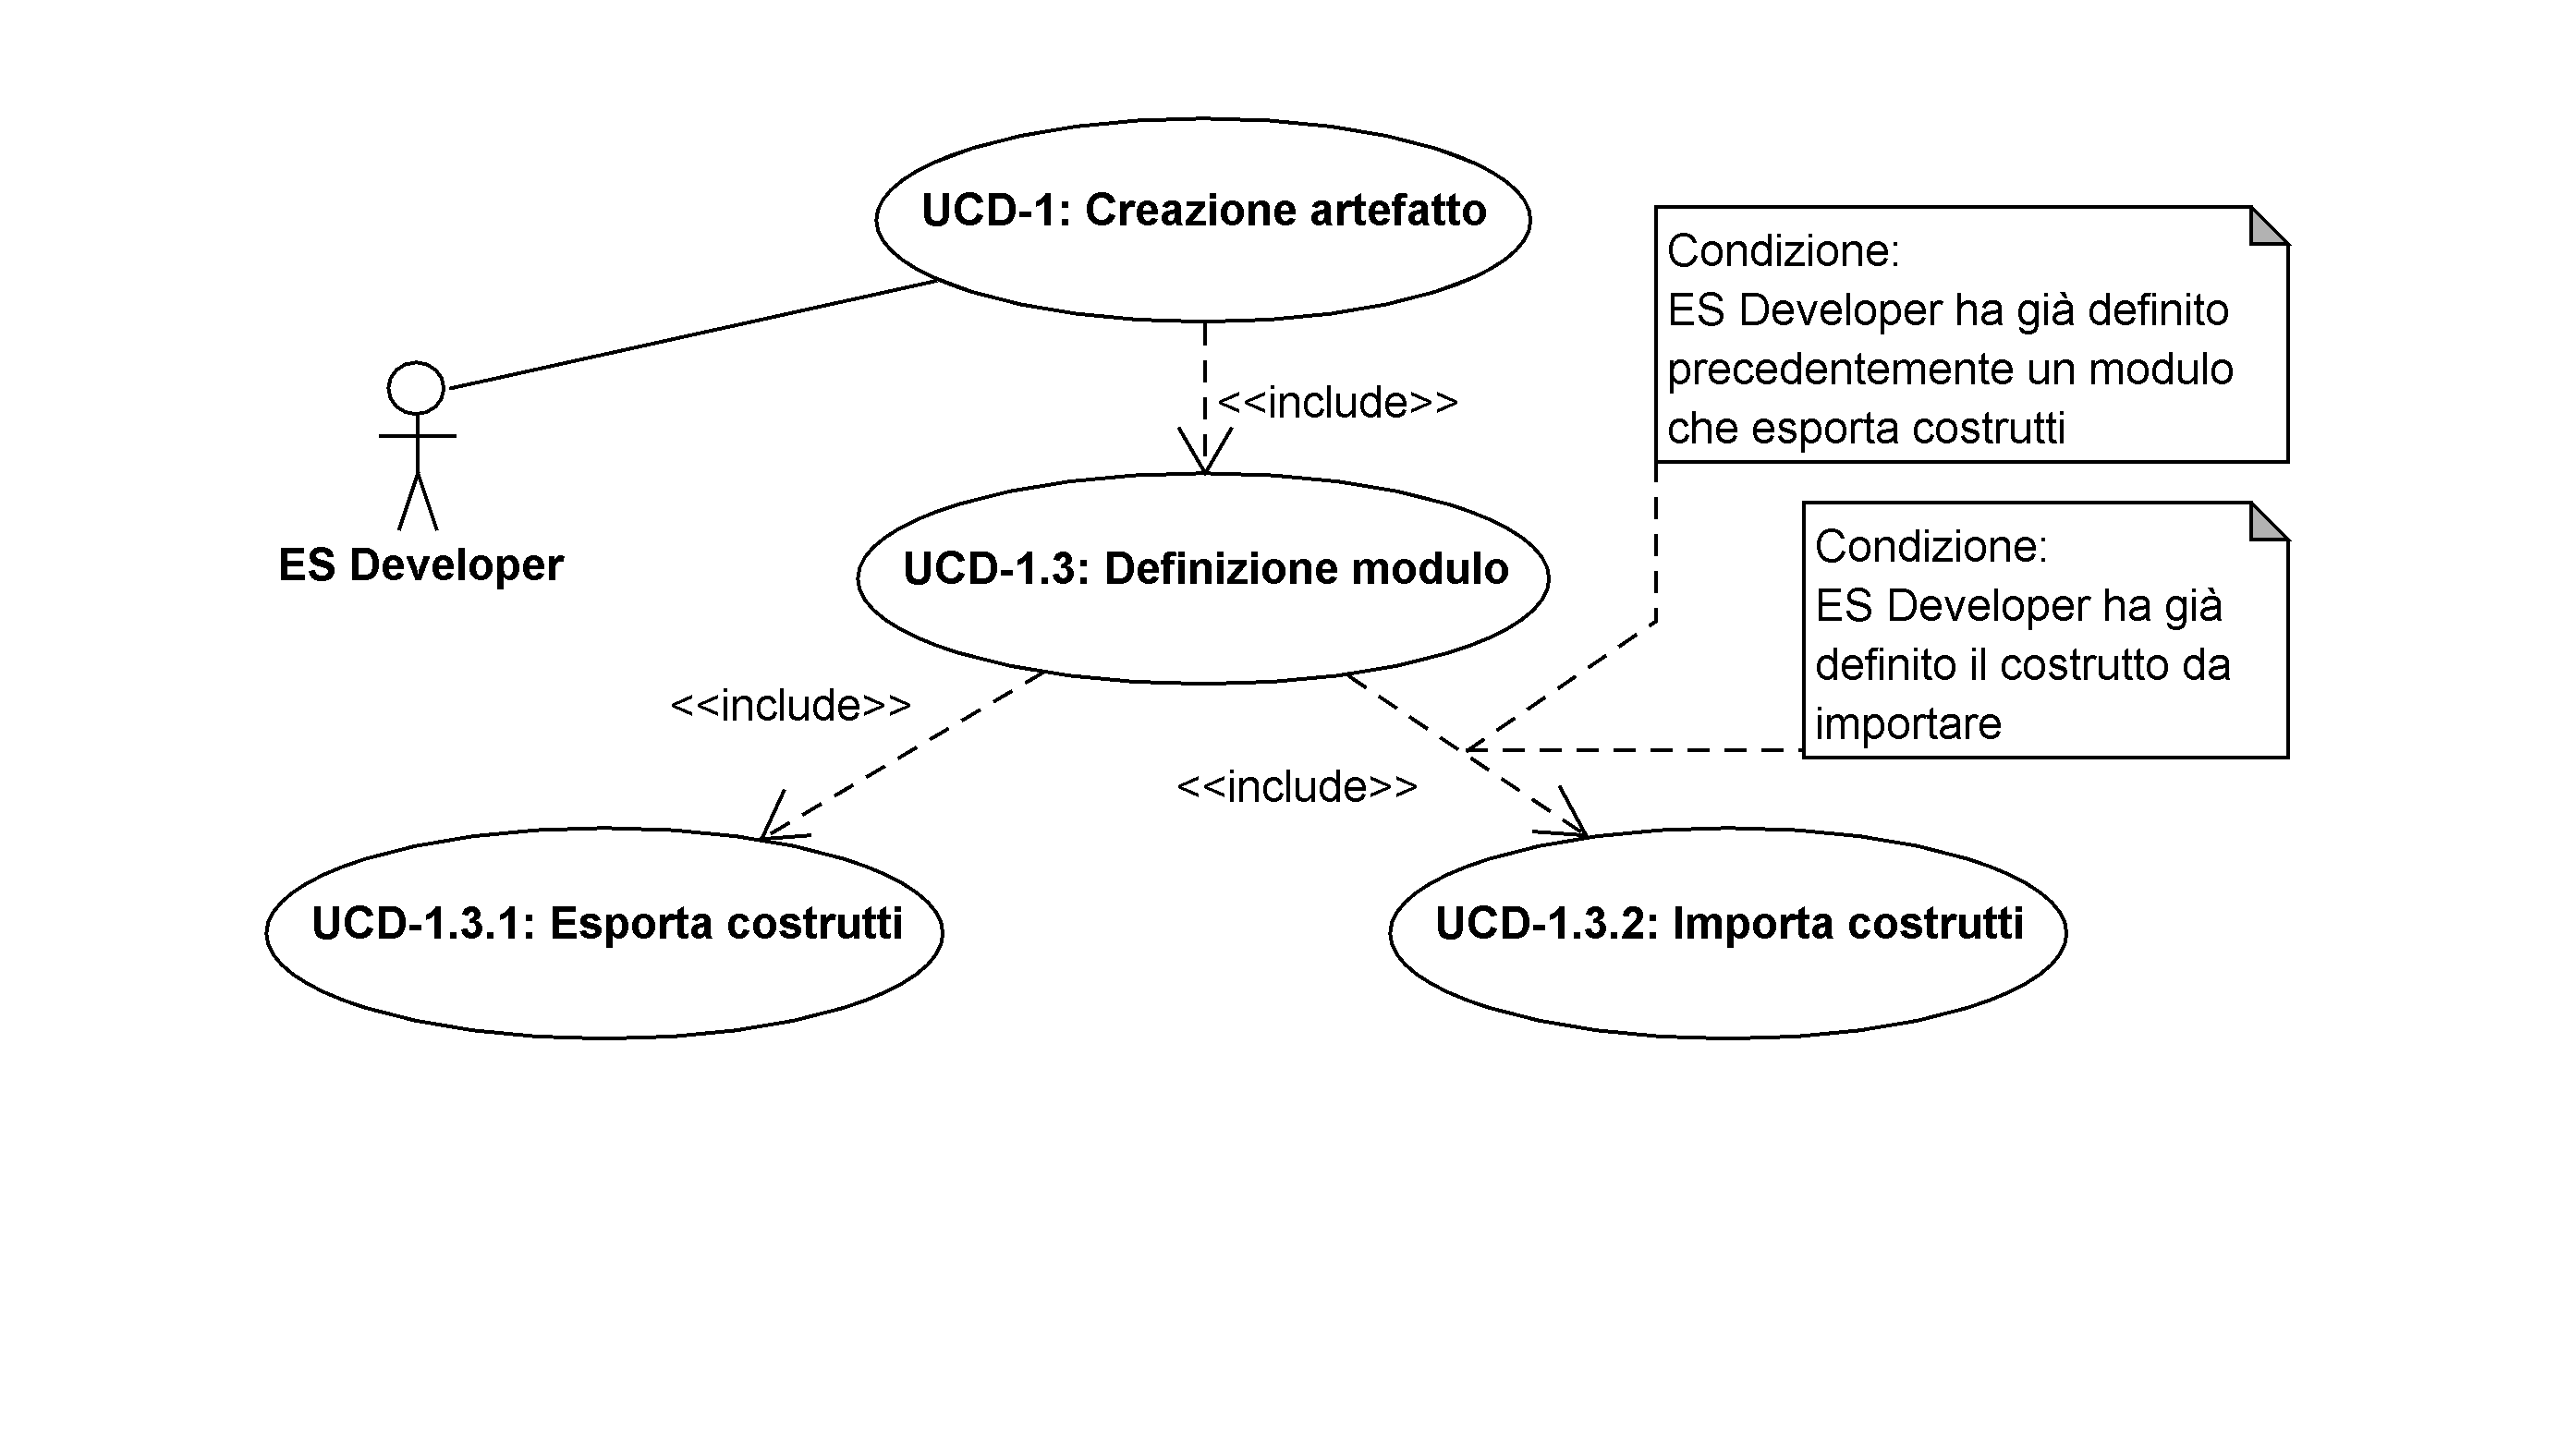
\includegraphics[width=1\textwidth]{Immagini/Capitolo2/UseCases/UCD-1_3.png}
\caption{Diagramma dei casi d'uso UCD-1.3}\label{fig:uc-ucd-1.3}
\end{figure}

\begin{itemize}
	\item \textbf{Attori:} ES Developer
	\item \textbf{Scopo e descrizione:} l'ES Developer deve essere in grado di definire un modulo tramite un linguaggio di specifica fornito dal sistema.
	\item \textbf{Pre-condizioni:} il software fornisce almeno un linguaggio di specifica.
	\item \textbf{Post-condizioni:} la definizione di un modulo è stata aggiunta ad un artefatto.
	\item \textbf{Flusso principale degli eventi:}
		\begin{enumerate}
			\item l'ES Developer definisce un modulo specificandone il nome
			\item l'ES Developer definisce una serie di costrutti da esportare (si veda il caso d'uso \emph{UCD-1.3.1})
			\item l'ES Developer definisce una serie di costrutti da importare da un altro modulo (si veda il caso d'uso \emph{UCD-1.3.2})
		\end{enumerate}
		
	\item \textbf{Flusso alternativo:} 
		\begin{enumerate}
			\setcounter{enumi}{0}
			\item se l'ES Developer fornisce un nome già utilizzato da un altro modulo, il sistema rifiuta la definizione e notifica l'errore.
			\item il sistema ritorna nello stato iniziale.
		\end{enumerate}
		
\end{itemize}

\subparagraph{UCD-1.3.1: Esporta costrutti}

\begin{itemize}
	\item \textbf{Attori:} ES Developer
	\item \textbf{Scopo e descrizione:} l'ES Developer deve essere in grado di specificare l'esportazione di un costrutto relativo al modulo tramite un linguaggio di specifica fornito dal sistema
	\item \textbf{Pre-condizioni:} il sistema fornisce un linguaggio di specifica, l'ES Developer ha definito un modulo
	\item \textbf{Post-condizioni:} il sistema aggiunge il nome del costrutto esportato in un insieme di elementi importabili da altri moduli
	\item \textbf{Flusso principale degli eventi:}
		\begin{enumerate}
			\item l'ES Developer definisce un modulo
			\item l'ES Developer definisce un costrutto appartenente al modulo come esportabile
				\begin{itemize}
					\item l'ES Developer può specificare il nome ed il tipo del costrutto
					\item l'ES Developer può specificare il tipo dei costrutti e un valore speciale per definire l'esportazione di tutti i costrutti del tipo indicato
					\item l'ES Developer può specificare un valore speciale per definire l'esportazione di tutti i costrutti di ogni tipo
					\item l'ES Developer può specificare il tipo ed un valore speciale per definire l'esclusione dei costrutti del tipo specificato dalla lista degli elementi esportati
				\end{itemize}
		\end{enumerate}
\end{itemize}


\subparagraph{UCD-1.3.2: Importa costrutti}

\begin{itemize}
	\item \textbf{Attori:} ES Developer
	\item \textbf{Scopo e descrizione:} l'ES Developer deve essere in grado di specificare l'importazione di un costrutto esportato da un modulo tramite un linguaggio di specifica fornito dal sistema
	\item \textbf{Pre-condizioni:} il sistema fornisce un linguaggio di specifica, l'ES Developer ha definito un modulo che esporta un costrutto, l'ES Developer ha definito un modulo
	\item \textbf{Post-condizioni:} il sistema aggiunge la definizione importata all'insieme di definizione del modulo.
	\item \textbf{Flusso principale degli eventi:}
		\begin{enumerate}
			\item l'ES Developer definisce un modulo
			\item l'ES Developer definisce un costrutto appartenente ad un secondo modulo come importabile.
				\begin{itemize}
					\item l'ES Developer può specificare il modulo, il nome ed il tipo del costrutto da importare
					\item l'ES Developer può specificare il modulo, il tipo ed un valore speciale per definite l'importazione di tutti i costrutti del tipo indicato dal modulo indicato
					\item l'ES Developer può specificare il modulo ed un valore speciale per definire l'importazione di tutti i costrutti dal modulo indicato
					
					\item l'ES Developer può specificare il modulo, il tipo ed un valore speciale per definire l'esclusione di tutti i costrutti del tipo indicato del modulo indicato dall'insieme di costrutti importati
				\end{itemize}
		\end{enumerate}
	\item \textbf{Flusso alternativo \#1:} 
		\begin{enumerate}
			\setcounter{enumi}{1}
			\item se l'ES Developer esegue un'importazione da un modulo non esistente, il sistema rifiuta la definizione e notifica l'errore.
			\item il sistema ritorna nello stato iniziale.
		\end{enumerate}
		
	\item \textbf{Flusso alternativo \#2:} 
		\begin{enumerate}
			\setcounter{enumi}{1}
			\item se l'ES Developer esegue un'importazione di un costrutto non ancora definito da un modulo che lo esporta preventivamente, il sistema rifiuta la definizione e notifica l'errore.
			\item il sistema ritorna nello stato iniziale.
		\end{enumerate}
		
\end{itemize}

\paragraph{UCD-1.4: Definizione fatti} % nome del caso d'uso Gruppo

\begin{figure}
\centering
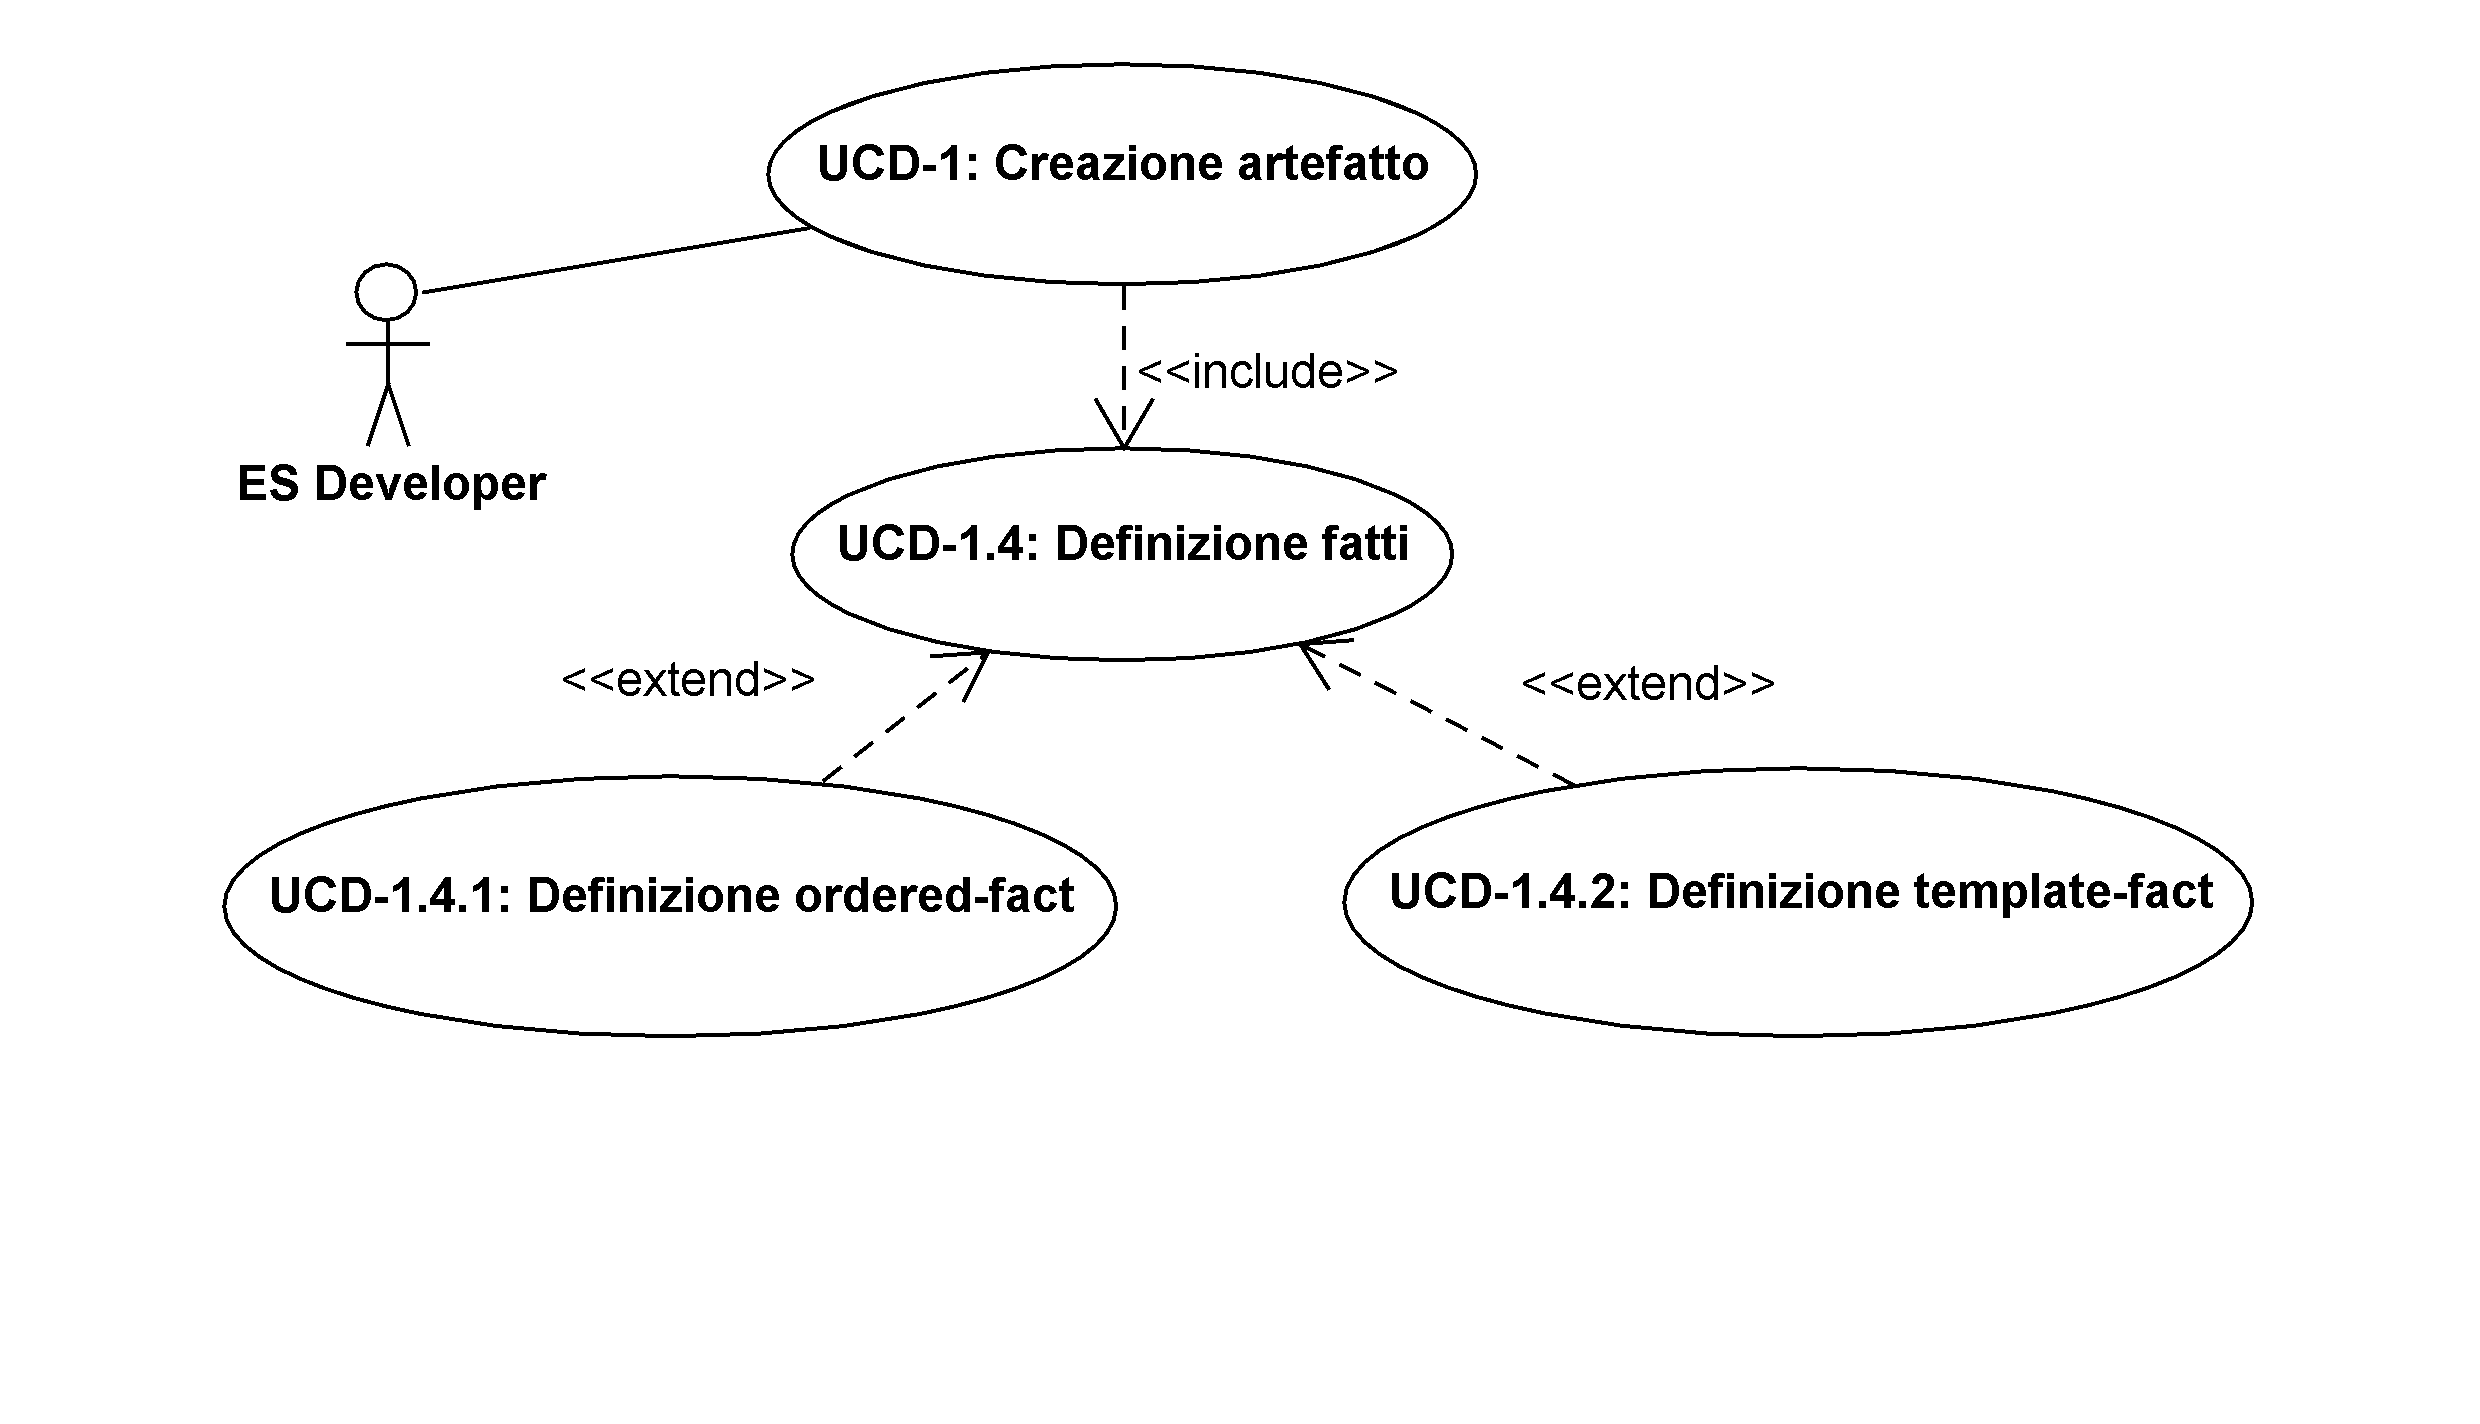
\includegraphics[width=1.1\textwidth]{Immagini/Capitolo2/UseCases/UCD-1_4.png}
\caption{Diagramma dei casi d'uso UCD-1.4}\label{fig:uc-ucd-1.4}
\end{figure}

\begin{itemize}
	\item \textbf{Attori:} ES Developer
	\item \textbf{Scopo e descrizione:} l'ES Developer deve essere in grado di definire un gruppo di fatti iniziali tramite un linguaggio di specifica fornito dal sistema
	\item \textbf{Pre-condizioni:} il software fornisce almeno un linguaggio di specifica
	\item \textbf{Post-condizioni:} la definizione del gruppo di fatti è stata aggiunta ad un artefatto
	\item \textbf{Flusso principale degli eventi:}
		\begin{enumerate}
			\item l'ES Developer definisce un gruppo di fatti specificando il nome
			\item l'ES Developer definisce una serie di fatti da associare al gruppo (si vedano i casi d'uso \emph{UCD-1.4.1} e \emph{UCD-1.4.2})
		\end{enumerate}
	\item \textbf{Flusso alternativo:}
		\begin{enumerate}
			\item se l'ES Developer ha definito precedentemente un modulo, l'ES Developer può definire il gruppo di fatti come componente del modulo.
			\item lo scenario prosegue dal punto 2 del flusso principale
		\end{enumerate}
\end{itemize}

\subparagraph{UCD-1.4.1: Definizione ordered-fact} % nome del caso d'uso SottoGruppo

\begin{itemize}
	\item \textbf{Attori:} ES Developer
	\item \textbf{Scopo e descrizione:}  l'ES Developer deve essere in grado di definire un fatto in notazione \emph{ordered-fact} tramite un linguaggio di specifica fornito dal sistema
	\item \textbf{Pre-condizioni:} il software fornisce almeno un linguaggio di specifica, l'ES Developer ha definito un gruppo di fatti iniziali
	\item \textbf{Post-condizioni:} il fatto in notazione \emph{ordered-fact} è aggiunto al gruppo di fatti iniziali
	\item \textbf{Flusso principale degli eventi:}
		\begin{enumerate}
			\item l'ES Developer definisce un gruppo di fatti iniziali
			\item l'ES Developer definisce un fatto in notazione \emph{ordered-fact} specificando l'elenco di componenti in sequenza
				\begin{itemize}
					\item l'ES Developer può specificare una sequenza di componenti di lunghezza arbitraria
					\item l'ES Developer può specificare una sequenza di componenti di tipo non omogeneo
				\end{itemize}
		\end{enumerate}
	\item \textbf{Flusso alternativo:}
		\begin{enumerate}
			\setcounter{enumi}{1}
			\item l'ES Developer definisce un fatto in notazione \emph{ordered-fact} con componenti identiche a quelle di un fatto specificato in precedenza
			\item il sistema ignora la definizione
		\end{enumerate}
\end{itemize}


\subparagraph{UCD-1.4.2: Definizione template-fact} % nome del caso d'uso SottoGruppo

\begin{itemize}
	\item \textbf{Attori:} ES Developer
	\item \textbf{Scopo e descrizione:}  l'ES Developer deve essere in grado di definire un fatto in notazione \emph{template-fact} tramite un linguaggio di specifica fornito dal sistema
	\item \textbf{Pre-condizioni:} il software fornisce almeno un linguaggio di specifica, l'ES Developer ha definito un gruppo di fatti iniziali
	\item \textbf{Post-condizioni:} il fatto in notazione \emph{template-fact} è aggiunto al gruppo di fatti iniziali
	\item \textbf{Flusso principale degli eventi:}
		\begin{enumerate}
			\item l'ES Developer definisce un gruppo di fatti iniziali
			\item l'ES Developer definisce un fatto in notazione \emph{template-fact} specificando il nome del \emph{template} di riferimento
			\item l'ES Developer definisce i valori degli slot (risp. multi-slot)
				\begin{itemize}
					\item l'ES Developer può specificare una sequenza di componenti di lunghezza arbitraria per i \emph{multi-slot}
					\item l'ES Developer può specificare un elemento per gli \emph{slot}
				\end{itemize}
			\item il sistema completa la definizione del fatto associando i valori di default agli \emph{slot} (risp. \emph{multi-slot}) non definiti.
		\end{enumerate}
	\item \textbf{Flusso alternativo \#1:}
		\begin{enumerate}
			\setcounter{enumi}{1}
			\item l'ES Developer fornisce un nome di template non valido
			\item il sistema rifiuta la definizione e notifica l'errore
			\item il sistema torna allo stato iniziale
		\end{enumerate}
	\item \textbf{Flusso alternativo \#2:}
		\begin{enumerate}
			\setcounter{enumi}{2}
			\item l'ES Developer assegna un valore ad uno \emph{slot} (risp. \emph{multi-slot}) non definito nella definizione del \emph{template}.
			\item il sistema rifiuta la definizione e notifica l'errore
			\item il sistema torna allo stato iniziale
		\end{enumerate}
\end{itemize}


\paragraph{UCD-1.5: Definizione variabile globale} % nome del caso d'uso Gruppo

\begin{itemize}
	\item \textbf{Attori:} ES Developer
	\item \textbf{Scopo e descrizione:}  l'ES Developer deve essere in grado di definire una variabile globale tramite un linguaggio di specifica.
	\item \textbf{Pre-condizioni:} il software fornisce almeno un linguaggio di specifica
	\item \textbf{Post-condizioni:} la definizione della variabile globale è stata aggiunta ad un artefatto
	\item \textbf{Flusso principale degli eventi:}
		\begin{enumerate}
			\item l'ES Developer definisce una variabile globale, indicando nome e valore iniziale
			\item il sistema valuta la definizione
		\end{enumerate}
	\item \textbf{Flusso alternativo \#1:} 
		\begin{enumerate}
			\setcounter{enumi}{1}
			\item se l'ES Developer ha indicato come nome per la variabile globale uno già utilizzato, il valore iniziale fornito viene sostituito a quello della definizione precedente
			\item lo scenario prosegue dal punto 2 del flusso principale
		\end{enumerate}
	\item \textbf{Flusso alternativo \#2:} 
		\begin{enumerate}
			\item se l'ES Developer ha definito precedentemente un modulo, l'ES Developer può definire la variabile globale come componente del modulo.
			\item lo scenario prosegue dal punto 2 del flusso principale
		\end{enumerate}
\end{itemize}

\paragraph{UCD-1.6: Definizione funzione} % nome del caso d'uso Gruppo

\begin{itemize}
	\item \textbf{Attori:} ES Developer
	\item \textbf{Scopo e descrizione:} l'ES Developer deve essere in grado di definire una funzione tramite un linguaggio di specifica
	\item \textbf{Pre-condizioni:} il software fornisce almeno un linguaggio di specifica
	\item \textbf{Post-condizioni:} la definizione della funzione è stata aggiunta ad un artefatto
	\item \textbf{Flusso principale degli eventi:}
		\begin{enumerate}
			\item l'ES Developer definisce una funzione utente, indicando nome, parametri e corpo della funzione
			\item il sistema valuta il nome della funzione
		\end{enumerate}
	\item \textbf{Flusso alternativo \#1:}
		\begin{enumerate}
			\setcounter{enumi}{1}
			\item se il nome fornito dall'ES Developer è già utilizzato da una definizione di funzione (di sistema o utente), il sistema rifiuta la definizione e notifica l'errore
			\item il sistema ritorna allo stato iniziale
		\end{enumerate}
	\item \textbf{Flusso alternativo \#2:}
		\begin{enumerate}
			\item se l'ES Developer ha definito precedentemente un modulo, l'ES Developer può definire la funzione utente come componente del modulo
			\item lo scenario procede dal punto 2 del flusso principale
		\end{enumerate}
\end{itemize}

